\documentclass[10pt,a4paper]{article}
\usepackage[utf8]{inputenc}
\usepackage[english]{babel}
\usepackage[square, numbers, sort&compress]{natbib}
\usepackage{graphicx}
\usepackage{float}
\usepackage{amsmath}
\usepackage{amsfonts}
\usepackage{amssymb}
\usepackage{media9}
\usepackage{color}
\definecolor{librellogreen}{RGB}{0,85,0}
\usepackage{fancyhdr}
\usepackage{lastpage}	
\usepackage{parskip}
\usepackage[scaled]{helvet}
\usepackage{blindtext}
\usepackage{sectsty}
\usepackage{multicol}
\usepackage{enumerate}
%\usepackage[svgnames]{xcolor}
\usepackage[labelfont={color=librellogreen,bf}, labelsep=period]{caption}
\renewcommand*{\familydefault}{\sfdefault}
\usepackage[left=1.75cm,right=1.75cm,top=1.75cm,bottom=3.75cm]{geometry}
\usepackage{titlesec}
\usepackage{svg}
\usepackage{flushend}
\PassOptionsToPackage{normalem}{ulem}
\usepackage{ulem}
	\providecolor{added}{rgb}{0,0,1}
	\providecolor{deleted}{rgb}{1,0,0}
	%% Change tracking with ulem
	\newcommand{\added}[1]{{\color{added}{}#1}}
	\newcommand{\deleted}[1]{{\color{deleted}\sout{#1}}}
\usepackage{setspace}
\usepackage[hyphens]{url}
\usepackage[hidelinks]{hyperref}
\urlstyle{same}
\raggedcolumns
\flushcolumns
\usepackage{etoolbox}
%\usepackage{caption}
\usepackage{supertabular}
\usepackage{booktabs}
\usepackage{microtype}
\usepackage{threeparttable}

\usepackage[color=yellow,icon=Comment,hoffset=-10mm, author=Librello Editorial's Office]{pdfcomment}

\titleformat{\section}
{\color{librellogreen}\normalfont\bfseries\filright}
{\color{librellogreen}\thesection.}{0.5em}{}

\titleformat{\subsection}
{\color{librellogreen}\normalfont\itshape\filright}
{\color{librellogreen}\thesubsection.}{0.5em}{}

\titleformat{\subsubsection}
{\color{librellogreen}\normalfont\itshape\filright}
{\color{librellogreen}\thesubsubsection.}{0.5em}{}

\usepackage{array} %criando coluna de largura fixa alinhada a esquerda
\newcolumntype{L}[1]{>{\raggedright\let\newline\\\arraybackslash\hspace{0pt}}p{#1}}
\renewcommand{\arraystretch}{1.3}
\titlespacing\section{0pt}{12pt}{12pt}
\titlespacing\subsection{0pt}{12pt}{12pt}
\titlespacing\subsubsection{0pt}{12pt}{12pt}	
\renewcommand*{\refname}{References and Notes}

\fancypagestyle{document}{
	\renewcommand{\footrulewidth}{0pt}
	\renewcommand{\headrulewidth}{0pt}
	\renewcommand{\footrulewidth}{0pt}
	\renewcommand{\headrulewidth}{0pt}
	\renewcommand{\footskip}{40pt}
	\cfoot{\normalfont\thepage}
	\rhead{}\lhead{}
}

\fancypagestyle{firstpage}{
	\renewcommand{\footrulewidth}{0pt}
	\renewcommand{\headrulewidth}{0pt}
	\renewcommand{\footrulewidth}{0pt}
	\renewcommand{\headrulewidth}{0pt}
	\renewcommand{\footskip}{70pt}
	\lhead{Challenges in Sustainability $\mid$ 2016 $\mid$ Volume 4 $\mid$ Issue 1 $\mid$ Pages \thepage--\pageref{LastPage} \\DOI: 10.12924/cis2016.04010003\\
	ISSN: 2297--6477}
	\rhead{\includegraphics[height=0.59in]{CiS.eps}}
	\lfoot{\footnotesize © 2016 by the authors; licensee Librello, Switzerland. This open access article was published\\ under a Creative Commons Attribution License (\url{http://creativecommons.org/licenses/by/4.0/}).}
	\cfoot{}
	\rfoot{\vspace*{-24pt}\includegraphics[height=0.49in]{librello.eps}}

}

\makeatletter
\def\NAT@def@citea{\def\@citea{\NAT@separator}}
\makeatother

\begin{document}
\flushcolumns
\raggedcolumns



\pagestyle{document}
\thispagestyle{firstpage}


\vspace*{70pt}

\setlength{\parindent}{0cm}
\textit{Research Article}
\vspace*{-12pt}

\begin{center}
\line(1,0){500}
\end{center}

\vspace*{12pt}
\begin{flushleft}
\begin{LARGE}
\textbf{{\color{librellogreen} Building Urban Agricultural Commons: A Utopia or a Reality?}}\\
\end{LARGE}

\vspace*{12pt}
Pierre Donadieu

\vspace*{6pt}

National School of Landscape Architecture of Versailles, Versailles, France. E-Mail: p.donadieu@ecole-paysage.fr;\\ Tel.: +33 139246200; Fax: +33 139246201

%\vspace*{6pt}

%* Corresponding author: E-Mail: bloch@zalf.de; Tel.: +49 3343282423; Fax: +49 3343282387\\
\vspace*{6pt}

Submitted: 29 January 2016 $\mid$ In revised form: 17 March 2016 $\mid$ Accepted: 20 March 2016 $\mid$\\
Published: 25 April 2016
\end{flushleft}
\setcounter{page}{3}


\vspace*{-18pt}
\begin{center}
\line(1,0){500}
\end{center}

\vspace*{12pt}
%\vspace{\baselineskip}

\begingroup\leftskip= 1cm\rightskip 1cm  

\textbf{{\color{librellogreen}Abstract:}} There are several categories of urban agriculture which need to be distinguished if we want to efficiently feed urban inhabitants with local agricultural produce while benefiting from other functions filled by urban agricultural landscapes: namely, eco-systemic functions or ecological and social functions. The second function will focus on methods to regulate unbuilt land in urban areas which have virtually no regulations and others which have strict controls preventing construction. The last will consist of possibilities to build, what I would refer to as, urban agricultural commons: in other words, tangible and intangible resources produced with farmers and gardeners for the inhabitants; for their local consumption and for the quality of the living environment, based on a political principle for common action. The concept of common is derived from the works of socioeconomist E. Ostrom (1990; \citep{r09}) and  French philosophers P. Dardot et C. Laval (2014; \citep{r01}): ``What is built in common''. It was applied to urban agriculture and landscape (Donadieu, 2012, 2014; \citep{r03, r04}). The concept of urban agriculture has been used worldwide in the last twenty years by researchers, especially in France by A. Fleury (2005; \citep{r07}) and P. Donadieu(1998; \citep{r02}), in Mediterranean regions (Nasr and Padilla, 2004; \citep{r11}), in Asia, Africa and North and South America---all through the publications of the Resource Centres  Urban Agriculture \& Food Security (RUAF; \citep{n01}).

\textbf{{\color{librellogreen}Keywords:}} multifunctional agriculture; urban agricultural commons; urban agriculture 
\par\endgroup
 
\setlength{\parindent}{0.5cm}
\setlength{\parskip}{0cm}
\setlength{\bibsep}{0cm}

\vspace*{10mm}
%\vspace*{20mm}

\begin{multicols}{2}

\section{Agrobusiness, Fun and Subsistence}
\subsection{Agrobusiness and Amateur Gardening}
\noindent There are two ways of producing food products around cities and for cities. The first, which is prevalent in terms of the number of producers, its economic weight and the surface area involved, concerns farmers and agricultural entrepreneurs. They produce for local markets (urban markets and shopping centres) or for more distant markets in the same country or abroad. They are market gardeners, wine growers, cereal growers, livestock farmers, nurserymen, etc. Some cultivate in fields and others cultivate in greenhouses. Their activity is a business, an agrobusiness. Some farmers receive support within the framework of the European Common Agricultural Policy and others, such as the livestock farmers, market gardeners and wine growers, receive little or none at all.

The second way of producing food products concerns amateur gardeners who represent a small proportion in terms of numbers and the surface area cultivated. They cultivate family allotments and community gardens and are to be found in much greater numbers in northern and central Europe than in the Mediterranean region. Their objective is not business but subsistence and/or leisure; the benefits of cultivating; of mutual support and the possibility of offering solidarity to those in need of help, such as the unemployed.

These agrobusinesses and amateur gardens occupy so-called open spaces: unbuilt spaces in urban areas, especially on the roofs of buildings, which provide the kinds of landscapes most appreciated by inhabitants. These agricultural and horticultural practices are often associated with woodlands, gardens, public and private parks and produce two types of urban agricultural landscapes. Subsistence landscapes are often regulated in the same way as in the north of Lisbon during the economic crisis (Figure \ref{Fig01}).

As regards leisure, enjoyment and pedagogical purposes, this is the case of Paris with its collective gardens (in French: \textit{jardins partagés}; \citep{n02}). There are more than one hundred collective gardens in Paris, situated next to residential buildings and in public parks and schools,  all of which are encouraged by town authorities. These are places which foster social interaction, but which also help people to re-establish a relationship with cultivated and natural environments. They can also provide opportunities to develop professional skills and often represent a lifeline for marginalised populations.

\vspace{\baselineskip}

\noindent
\begin{minipage}{\columnwidth}
\centering
\resizebox{\columnwidth}{!}
{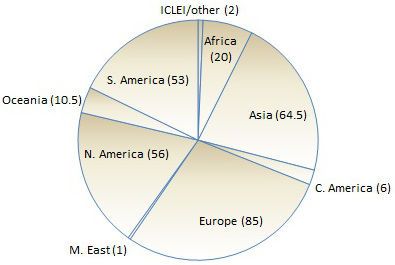
\includegraphics[width=\textwidth]{Fig01.jpg}}
\captionof{figure}{Community gardens in the north of Lisbon (Portugal). \label{Fig01}}
\end{minipage}

\subsection{An Urban Agricultural Order: A Paradigm Shift?}
\noindent Public authority interventions vary depending on political situations. In Switzerland, city authorities sometimes cover the costs of production sites, as in the case of the vineyard of the Lausanne City Farm, or of urban farmland in Geneva which has been protected from urban development since the 1960s (Figure \ref{Fig02}).

Urban authorities and many inhabitants dislike anything that evokes disorder, insecurity or poverty, such as improvised gardening sheds built by gardeners. In France, people like orderly family allotment gardens such as those set up in the new town of Saint Quentin-en-Yvelines, near Versailles, in 1985, or in a public garden in Angers in 2002 (Figure \ref{Fig03}).

But for the main part, the urban agricultural order is the one produced by private agricultural enterprises on land, generally poorly protected from urbanisation. In France an average of 50,000 hectares of agricultural land disappears every year. Legal protection systems exist in almost all European countries but they insufficiently contain the pressure of urbanisation. In France, building permits given by the public authorities increases the value of land by 10 to 100. Only a strong political will, high environmental risks, extremely strong legal protection or exceptional profits from wine production (as in the region of Bordeaux,  France) are able to contain urban sprawl.

In the end, the issue for elected representatives, specialists and the inhabitants of urban areas is quite simple: how to choose beyond the alternative between, the landowners' right of disposing of agricultural land, and the construction of urban public agricultural areas on private or public land? 

The urban agricultural commons I am referring to are not public property, they are not community property either since they fall outside the scope of both categories. They are what is built in common for a general interest: the use of fertile agricultural and gardening land to grow food and fulfil sustainable local functions.

\vspace{\baselineskip}

\noindent
\begin{minipage}{\columnwidth}
\centering
\resizebox{0.85\columnwidth}{!}
{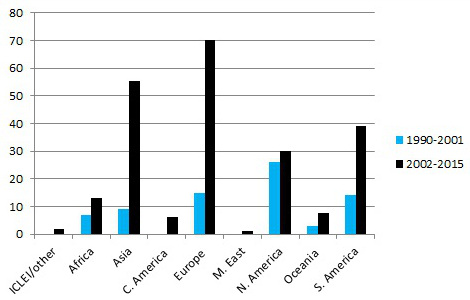
\includegraphics[width=0.85\textwidth]{Fig02.jpg}}
\captionof{figure}{Vinyard of the Lausanne City Farm (Switzerland), near the Leman lake. \label{Fig02}}
\end{minipage}

\vspace{\baselineskip}

\noindent
\begin{minipage}{\columnwidth}
\centering
\resizebox{\columnwidth}{!}
{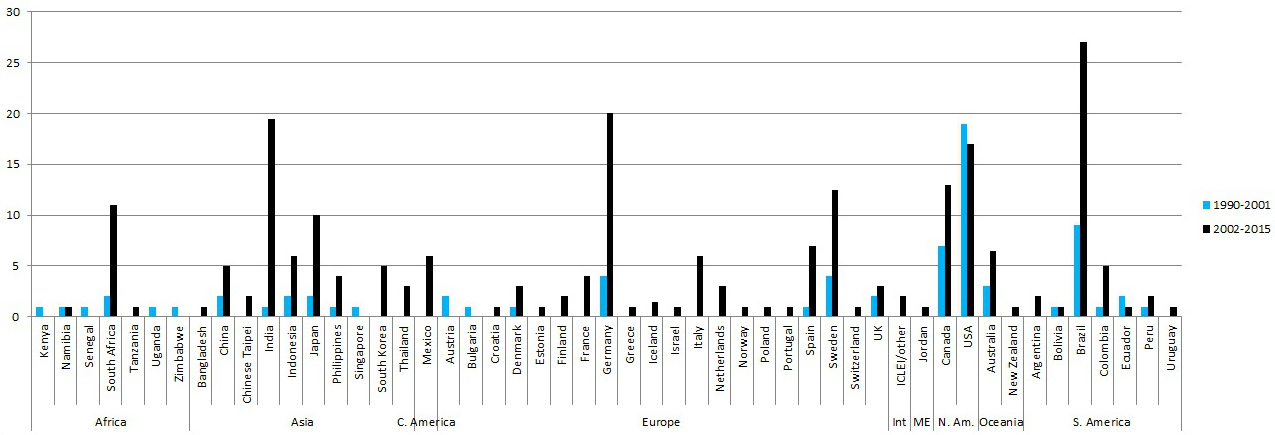
\includegraphics[width=\textwidth]{Fig03.jpg}}
\captionof{figure}{Community gardens in a public park, in the center of Angers (Loire Valley, west France). \label{Fig03}}
\end{minipage}

\clearpage

This is a revolution, a radical paradigm shift because it requires insurance that the cultivated land, the crops and livestock produced, and the farmers provide sustainable urban resources. These resources should not be evicted from the city as that has been the case during more than a century of hygienic modernism, an ethical principle which has undoubtedly become obsolete. That is why a more pragmatic approach, which  takes potential impacts into account, is to be recommended: to ensure that everyone benefits from the eco-systemic goods provided by a diversified urban agriculture. To choose and prioritise them, because all eco-systemic supply, regulation and cultivation services cannot be provided equally to all the inhabitants. Because they are not just consumers but also inhabitants who want to enjoy a good quality of life in their own environment.  

\subsection{The Urban Region: A New Vision of the City}
\noindent The old-fashioned, so-called modern city, invented in the 20th century is no longer viable. There is a need to invent another model based on the simple notion that all urban planners and landscape architects are familiar with: the system of parks developed by Frederick Law Olmsted in the United States and Jean-Claude Nicolas Forestier in France at the end of the 19th century. An urban agricultural system of public parks which includes future agricultural and gardening spaces. They are referred to as ecological networks or, in France, green and aquatic networks (in French: \textit{trame verte et aquatique}). These parks are designed at the city level following the scientific research in landscape ecology conducted by Richard Forman and Michel Godron on the conditions to restore biodiversity. These unbuilt areas provide indispensable eco-systemic functions for the city: agriculture for food and energy, vegetation to regulate urban microclimates, the regulation of environmental risks (floods, fire, erosion of biodiversity, pollution of water tables) and the sequestration in the soil and the vegetation of excess carbon in the air.

The development of urban agriculture should be associated with policies for ecological networks and biodiversity as well as other public policies such as those relating to energy. These practices and policies are being deployed in Europe, but the pace is slowing due to the need for housing which irreversibly occupies too much valuable farmland. Is it possible to resort to other than regulatory means to preserve agricultural land, for instance by revisiting the notion of the common?

\section{The Building of Urban Agricultural Commons}
\subsection{The Destruction of the Commons: An Old Socio-Political Process}
\noindent \textls[-5]{Agricultural activity is not the result of nature but of culture, in the sense of cultivation for food and energy along with the cultural values attributed to such production. That is why the spaces and the tools used in agriculture have never been res nullius: things belonging to no one, such as the air or the fish in the sea. The use of land for farming automatically engenders its appropriation as well as that of its produce, at least during the cultivation or production cycle \citep{r02}.}

So much so that in the cases of traditional African societies or of the former European commons, the land is jointly owned by the community; the modern legal notion of the individual ownership of land (\textit{usus, fructus et abusus}) does not apply. It is the representatives of the community who decide on the collective rules governing the use of the land for crop or livestock farming. In such a context, which still applies in pastoral societies, the land and its permanent plant cover is \textit{res communis}, public domain, a common resource, accessible to the rights holders of the community (a village, a municipality, an ethnic group). If the rules for the conservation of natural resources (soil, grass, tree, water) are not respected, the resource is put at risk and may even disappear: as a result its shared use is jeopardised (this is the ``Tragedy of the Commons'' theorised by the American economist Garett Hardin in the 1960s \citep{r12}).

In such conditions two solutions are adopted: the land is privatised (\textit{res privata}) by the sharing of the land between the right holders with or without the enclosure of the plots (as in the case of the enclosures in England in the 18th century), or it is made a public property: \textit{res publica} (by allocating it as a part of the public domain of local authorities).

In the urban environment, collective property may persist as in the case of the commons in English cities (green, non-agricultural public spaces open to the public). Generally, unbuilt, wooded, agricultural land or aquatic spaces are either privately owned or the property of the State. Common lands have practically disappeared from the two categories defined by economists: public properties (in principle outside the realm of the market), and properties accessible via the market: property belonging to clubs (payment of a fee without exclusion) and exclusive private property.

\subsection{The Construction of Agricultural Urban Commons: A Socio-Political Form of Governance}
\noindent As demonstrated by the economist Elinor Ostrom (1933--2012), it is possible to create and preserve common resources (the water from water tables---in Los Angeles especially---an irrigation system, the fish in the sea) and to transmit them in good conditions. Such rational governance of a resource also applies to unbuilt lands in urban areas. It mobilises land owners, the users of ``natural'' soils (farmers, foresters, naturalists) or artificial soils (hydroponic farms), public authorities, experts, and generally ``the public'', as defined by the American pragmatist philosopher John Dewey (1859--1962). The governance stakeholders, the ``appropriators'' and the public authorities, define the rules for the use of productive public or private agricultural and urban land. In post-industrial dross and brownfields sites, soils are often polluted. In France, the creation of community gardens requires a joint project between public authorities and gardeners \citep{r05}.

A common is therefore a political principle of deliberation, of co-decision and action. The things built in common become common to the actor and co-deciders, ``that which is covered by the activity of putting something in common, that which is produced in common by this activity'' \citep{r01}. This common practice designates things, objects, private or public (the soil and the plants, farm produce and forestry products), and an awareness of moral values (justice, solidarity, freedom, dignity, etc.) which are at the basis of collective deliberation (co-decision). We shall call them agricultural urban commons.

\textls[25]{They adopt different forms according to local histories. On the Saclay plateau to the West of Paris, near Versailles, 2,000 hectares of private agricultural land farmed by 12 farmers have been protected from urbanisation (listed under a law for the protection of sites) in 2000 (Figure \ref{Fig04}).}

\vspace{2\baselineskip}

\noindent
\begin{minipage}{\columnwidth}
\centering
\resizebox{\columnwidth}{!}
{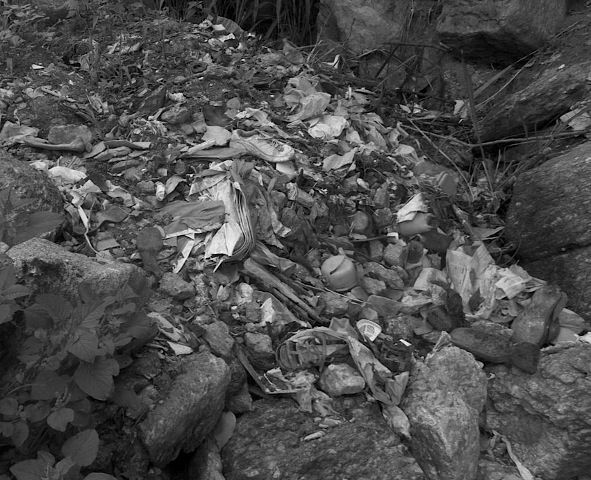
\includegraphics[width=\textwidth]{Fig04.png}}
\captionof{figure}{``The Plateau de Saclay'', near Versailles (France), rapeseed crops and orchards. \label{Fig04}}
\end{minipage}

\columnbreak

\textls[-25]{This land and its cereal farming landscapes have become the commons of the inhabitants of the plateau; students and teachers from the Paris Saclay University campus; a branch of the French national agency of research in agronomy (INRA, or National Institute of Agricultural Research); the grouping of municipalities of Saint-Quentin-en-Yvelines; local public; private real estate organisations and the State (Paris-Saclay Public Land Agency since 2010). The agricultural urban commons of the Saclay Plateau were established by a system of territorial governance which emerged in the 1970s as a result of environmental demands expressed by the inhabitants.}

\textls[-15]{The same thing occurred in the case of the Plaine de Versailles where a surface area of 2,000 hectares was protected by a territorial governance body composed of the grouping of municipalities of Versailles Grand Parc, and the association of farmers, elected representatives, inhabitants and public agencies of the Chateau de Versailles area (Figure \ref{Fig05}).}

\textls[-25]{When public or private institutions are confronted with the democratic expression of territorial stakeholders and with the tensions and conflicts caused by competition between building (housing, commercial zones, leisure areas) and food production, the ensuing discussions result in the creation of a common. In certain cases, such as Saclay, associations of consumers take ownership of land with the aim of producing local organic farm produce. In other areas, such as the Rennes metropolis (West France), the notion of \textit{urban fields} designates land open to an agricultural and urban multi-functionality. Common projects fail, however, if stakeholders do not agree. These agreements often require a lot of time and are not eternal!}

\textls[-25]{These new commons designate agricultural spaces which are usually private and the agricultural use of which is decided by, and for, local stakeholders and inhabitants who support their preservation. These spaces are similar to classic ``commons'' because they can be exhausted as a result of urban sprawl, but they are different in that they are appropriated. It is therefore common action which produces the common and not the over-abundance or inability to appropriate the resource (such as the air or the sea). Therefore, a soil, the function and agricultural uses of which fulfil eco-systemic functions (production, regulation, transmission) recognised as useful by the inhabitants, becomes a common.}

\vspace{\baselineskip}

\noindent
\begin{minipage}{\columnwidth}
\centering
\resizebox{\columnwidth}{!}
{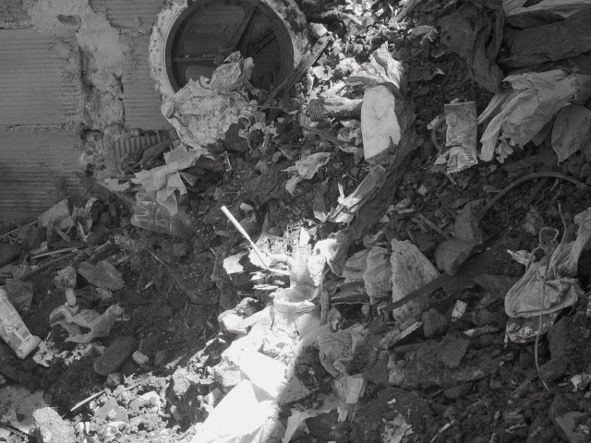
\includegraphics[width=\textwidth]{Fig05.jpg}}
\captionof{figure}{Gally farms, near the Castle of Versailles. Strawberry crops under shelter. \label{Fig05}}
\end{minipage}

These ``edaphic'' commons become assets when entitled persons are allowed to defend their transmission. In such a case, the stakeholders of this transformation into an asset are public agencies (such as land and urban planning agencies), private entities (owners and tenants) and the users who have access to the sites (for purposes of leisure or direct supply). 

\subsection{Organising Urban Growth and the Preservation of Open Spaces}
\noindent An essential priority for the possible existence of agricultural urban commons is the conservation of cultivable and wooded land according to geographic continuities. It starts with the cartographic indication of the desirable use of the land in urban planning documents. For at least forty years the Ile-de-France region has had an urban planning policy. Initially it did not cover agricultural spaces, but today it includes a regional plan for open (unbuilt) agricultural and forestry spaces, which provides a political framework for the actions of elected representatives in municipalities. In addition, the policy for regional land use management (in French: \textit{Périmètres Régionaux d’Intervention Foncière}, PRIF) make it possible for the agency in charge of green spaces (in French: \textit{Agence des espaces verts}) to buy threatened agricultural land and nature areas. The same applies for all the municipalities which have had a territorial development master plan for the last ten years such as the grouping of agglomerations of Montpellier (since 2004).

Within this legal framework, which is clearly in favour of the general interest (the shared objective of providing healthy local food), it is very difficult for elected representatives to prevent the urbanisation of open spaces and advocate for reasoned agricultural urbanism. What forms of agriculture do urban municipalities need? This is a second essential issue.

\subsection{Vertical or Horizontal Urban Farms?}
\noindent For fifteen years now it has been theoretically possible to build vertical farms or production units. These essentially use the hydroponic farming model which is perfectly mastered by horticultural farmers, especially in green houses. Investors, however, have remained very cautious and so far hardly any vertical constructions have seen the light of day.

That is why the conventional solution of horizontal farms situated in urban green areas is far preferable, as seen in a recent project (2009) in Munich,  Germany. These farms already exist, such as the orchards and large dairy farm of Viltain on the Saclay Plateau. With a few conditions: compliance with principles guiding ethical ecological agricultural, and in some cases, local production: animal welfare, limited or proscribed use of pesticides, organic farming, short farm-to-market cycles, organised access for the public, etc.

Another condition is that farmers should find in these continuous agricultural spaces few of the problems that might urge them to move away from cities: problems with the circulation of farm vehicles and machines on clean roads, problems with sources of organic matter (livestock, compost), the lack of local technical and veterinary assistance or of storage buildings and, above all, the possibility of transforming their crops and produce locally.

A last condition is that in the medium term there should be no uncertainty concerning the continued use of the land for farming. Farmers investing in agriculture cannot buy machines and animals, work on fertilising soils and selecting crops and deciding on which ones to rotate, develop quality produce and gain the confidence of clients if they have no control over the land through ownership or rental. In this area European countries have very different legislation which makes it possible to develop the use of unbuilt lands as commons. For mainly environmental (biodiversity) but also food production reasons there are private and public land agencies which make it possible to build urban agricultural and forestry networks. This is the case in France, for example, with the land development and farming societies (in French: \textit{Société d’aménagement foncier et d’établissement agricole}, SAFER), or the green space agencies (in French: \textit{Agence des espaces verts}) in the Ile-de-France region. But all these tools are unable to prevent the consumption of agricultural land.

The ideal solution would be to ensure that agricultural land and the use of agricultural urban commons should become as “natural” as urban forests and public parks and gardens in the minds of everyone. Since such a utopian point of view is not feasible there is a need for a pragmatic approach: to experiment and evaluate the results with the inhabitants, elected representatives and farmers, and to improve practises and new projects for the benefit of all.

\subsection{Which Form of Territorial Agricultural Urban Governance?}
\noindent \textls[-15]{So that an agricultural urban environment can actually exist, the political will to develop and share it with the people concerned is a prerequisite. The urban area of Rennes in the west of France (400,000 inhabitants) is a fine example. For almost 20 years, its elected representatives have sought to build with urban planners, farmers and landscape architects an urban agricultural region in the form of an archipelago; in other words, urban islands localised in a woody landscape of Brittany (in French: \textit{bocage}), a network of small towns and a centre linked by road and rail (metro) infrastructures. This vision of a rural city, or urban countryside, was shared by local politicians and inhabitants. And farmers are grouped together to sell their livestock and vegetable produce. The inhabitants of this city live in an urban area in which farming activities are a part of the urban environment, where urban planners have designed green and aquatic networks, pedestrian and cycling lanes, and where chambers of agriculture have supported the development of short cycles to bring produce to market and organised the production and processing sectors. Tensions subsist, namely in the land property market, but the notion of an urban agricultural region has become a reality.}

Another significant trend has developed during the last thirty years in Europe by which consumers pick produce directly from the farm, such as in the urban region of Versailles Grand Parc on the Gally Farm (Figure \ref{Fig06}).

 There is currently a plan for the installation of a similar farm gate direct marketing operation in Monza, North of Milan. It is the shortest channel to market for produce where the producer is directly in contact with the consumer and which also provides a pleasant experience of country life. Initially, crop varieties were limited, but the variety of cultivated species has considerably increased today, some cases including as many as 50 or 60 different species in efforts to address the increase in demand.
 
I could mention other urban agricultural practices indicating the existence of significant urban agricultural activity: greenhouse farming, riding centers, agritourism and bee-keeping in town.
Sometimes inhabitants are invited to farms to participate in wine harvesting, as in the North of Montpellier (South France) in a vineyard belonging to the urban community. Such pleasant activities would be difficult to imagine in sterile vertical farms.

Access to community gardens close to one’s urban residence has become a form of luxury that the city of Versailles is promoting in working-class neighbourhoods. The possibility of meeting one’s gardening neighbours, of engaging in a social activity which also puts one in contact with nature, with the land, and procures the pleasure of consuming one's own vegetables: these are valuable commons local inhabitants have benefited from since World War Two. These commons also provide wages for 150 people within the framework of a social insertion program. Could vertical farms provide such community services?

To be able to admire the countryside while living and moving about town, these are sensations urban planners have deprived European urban inhabitants of since the end of the 19th century. For instance, in the Netherlands, near Rotterdam, a typical example of an urban country, the population is not deprived of the joys of spring thanks to the presence of vast fields of bluebells.

Another idea related to sustainable development, which is becoming widespread today in metropolitan areas, is the notion of self-sufficiency for the most fragile types of produce such as fresh produce. In order to achieve this in the metropolitan area of Rennes, all green spaces would probably have to be converted to agriculture which would not be desirable except in an exceptional circumstance such as a war. Finally, we must remember that green spaces have often in the past been used to exclude the use of poor or marginalised populations. Today,  the challenge of the commons is to build an alternative to the private use of public spaces \citep{r08}.

\section{Conclusion}
\noindent In this new context, to compose or design the agricultural city and to give it new forms is a challenge for the landscape architects and urban planners of the 21st century. This practice existed in France when Louis XIV asked the architect Mansart and the gardener Jean-Baptiste de la Quintinie to install a vegetable garden and orchard of 12 hectares next to his palace in the new town of Versailles. Why not mobilise these competences again (Figure \ref{Fig07})?

Why not design an urban agricultural environment with the tools and concepts of landscape architecture? This would involve showcasing agricultural activities ranging from the most high-tech to the most traditional, and highlighting and promoting their social, economic, environmental and cultural benefits. It happens to be the complete opposite of what was done during the 20th century. This would undoubtedly make it possible for such activities to be accessible to a majority of the population!

The sharing of agricultural or garden land and products through a form of territorial governance is not a utopian dream. However, it is idealistic in that it challenges the consumer's model of society and notably, the fact of supplying cities by means of long-distance transport with its repercussions on energy consumption and public health in a context of increasing food insecurity. And yet, such a notion is realistic as the examples cited above demonstrate.

Utopias like vertical farms are probably chimerical---to bring all the food necessary for the city dwellers. ``Horizontal'' urban farming on natural or artificial soils for, and with consumers, is a better solution.  The notion of the common is a political principle and a shared duty for stakeholders such as public authorities and associations as well as private organisations and individuals engaged in the same activity: the creation and conservation of local farming and gardening activities on cultivated lands which can be transformed into urban assets. 

\vspace{\baselineskip}

\noindent
\begin{minipage}{\columnwidth}
\centering
\resizebox{0.9\columnwidth}{!}
{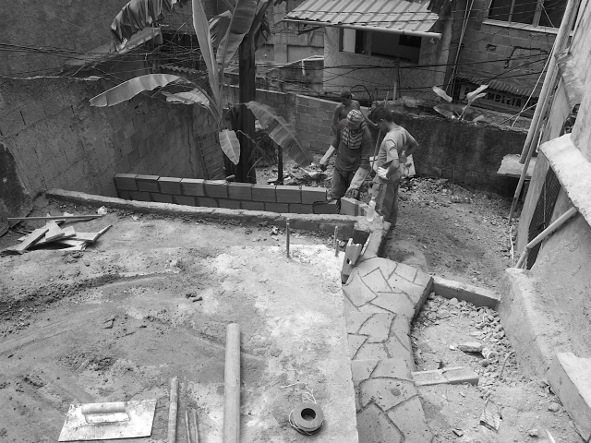
\includegraphics[width=0.9\textwidth]{Fig06.png}}
\captionof{figure}{Direct picking, Gally farms, Urban region of Versailles (West Paris). \label{Fig06}}
\end{minipage}

\vspace{\baselineskip}

\noindent
\begin{minipage}{\columnwidth}
\centering
\resizebox{\columnwidth}{!}
{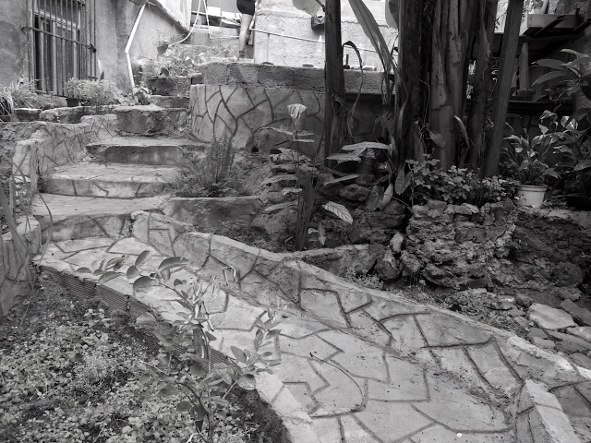
\includegraphics[width=\textwidth]{Fig07.jpg}}
\captionof{figure}{The \textit{Potager du Roi}, Versailles. \label{Fig07}}
\end{minipage}

\end{multicols}

\vspace{\baselineskip}

\begin{multicols}{2}
\renewcommand*{\refname}{References and Notes}

\bibliographystyle{vancouver}
%\bibliography{255-Biblio.bib}

\begin{thebibliography}{10}

\bibitem{r09}
Ostrom E.
\newblock Governing the commons: The evolution of institutions for collective
  action.
\newblock Cambridge, UK: Cambridge University Press; 1990.

\bibitem{r01}
Dardot P, Laval C.
\newblock Commun: essai sur la r{\'e}volution au XXIe si{\`e}cle.
\newblock Paris, France: la D{\'e}couverte; 2015.

\bibitem{r03}
Donadieu P.
\newblock Sciences du paysage: entre th{\'e}ories et pratiques.
\newblock Paris, France: Lavoisier; 2012.

\bibitem{r04}
Donadieu P.
\newblock Paysages en commun. Pour une {\'e}thique des mondes v{\'e}cus.
\newblock Presses Universitaires de Valenciennes; 2014.

\bibitem{r07}
Fleury A.
\newblock Multifonctionnalit{\'e} de l'agriculture p{\'e}riurbaine: vers une
  agriculture du projet urbain.
\newblock 5. INRA-CEMAGREF-CIRAD; 2005.

\bibitem{r02}
Donadieu P.
\newblock Campagnes Urbaines.
\newblock Arles, France: Actes Sud; 1998.

\bibitem{r11}
\textls[-25]{Nasr J, Padilla M.
\newblock Interfaces: agricultures et villes {\`a} l'Est et au Sud de la
  M{\'e}diterran{\'e}e.
\newblock Guildford, UK: Delta; 2004.}

\bibitem{n01}
Resource Centres Urban Agriculture \& Food Security (RUAF);.
\newblock Available from:
  \url{http://www.ruaf.org/publications/books-and-papers}.

\bibitem{n02}
\textls[-45]{See:
  \url{http://www.paris.fr/services-et-infos-pratiques/environnement-et-espaces-verts/nature-et-espaces-verts/les-jardins-partages-203}.}
  The gardens of associations of dwellers are often located on plots of the
  city of Paris.

\bibitem{r12}
Hardin G.
\newblock The tragedy of the commons.
\newblock science. 1968;162(3859):1243--1248.

\bibitem{r05}
Donadieu P, Remy E, Girard MC.
\newblock Les sols peuvent-ils devenir des biens communs?
\newblock Nature, Science, Société. \textit{in press}.

\bibitem{r08}
Harvey D, Le~Roy C, Vieillescazes N, Garrot C.
\newblock Le capitalisme contre le droit {\`a} la ville:
  N{\'e}olib{\'e}ralisme, urbanisation, r{\'e}sistances.
\newblock Paris, France: Ed. Amsterdam; 2011.

\end{thebibliography}





\end{multicols}


\end{document}




